\documentclass[12pt,twoside]{article}
\usepackage[a4paper, margin=1in]{geometry}
\usepackage{amsmath}
\usepackage[spanish]{babel}
\usepackage[active]{srcltx}
\usepackage{amssymb}
\usepackage{amscd}
\usepackage{makeidx}
\usepackage{amsthm}
\usepackage{algorithm}
\usepackage{amssymb, amsmath}
\usepackage[utf8]{inputenc}
\usepackage{fancyhdr}
\usepackage{graphics}
\usepackage{amsmath, amssymb}
\usepackage{amsmath}
\usepackage{listings}
\usepackage{xcolor}
\usepackage{fancyhdr}
\usepackage[active]{srcltx}
\usepackage{amsmath}
\usepackage{amssymb}
\usepackage{amscd}
\usepackage{makeidx}
\usepackage{graphicx}
\usepackage{caption}
\usepackage{url}
\usepackage{enumitem}
\usepackage{fancybox}
\usepackage{tabularx}

\renewcommand{\baselinestretch}{1}
\setcounter{page}{1}
\setlength{\textheight}{21.6cm}
\setlength{\textwidth}{14cm}
\setlength{\oddsidemargin}{1cm}
\setlength{\evensidemargin}{1cm}
\pagestyle{myheadings}
\thispagestyle{empty}
\markboth{\small{Ecos Team}}{\small{Formulación del Proyecto}}
\date{} 

\begin{document}
	
	\begin{center}
		
		% Contenido izquierdo - Imagen
		\begin{minipage}{0.17\textwidth}
			\flushleft
			
\includegraphics[width=0.9\textwidth]{img/ipn_logo.png} % Ajusta esta línea
		\end{minipage}
		\begin{minipage}{.55\textwidth}
			\centering
			{\Large Instituto Politécnico Nacional}\\
			{\Large Escuela Superior de Cómputo}
		\end{minipage}
		\begin{minipage}{0.17\textwidth}
			\flushright
			
\includegraphics[width=0.9\textwidth]{img/escom_logo} % Ajusta esta línea
		\end{minipage}			
	\end{center}
	
	
	\centerline{\bf Ingeniería en Inteligencia Artificial, Análisis y diseño de sistemas}
	
	\centerline{\bf Sem: 2024-2, 4BM2, Reporte técnico, Fecha: 27-06-24\\\\}
	
	\centerline{}
	
	%\centerline{}
	
	
	\begin{center}
		\Large{\textsc{Ecos del alma: Prototipo de juego rogue lite con interacción jugador-NPC dinámica}} 
	\end{center}
	\centerline{}
	\centerline{\bf {\textit{Presentan}}}
	\centerline{}
	\centerline{\bf {Angeles López Erick Jesse\footnote{eangelesl1700@alumno.ipn.mx}}}
	\centerline{\bf {Corona Anchondo José Antonio\footnote{jcoronaa1900@alumno.ipn.mx}}}
	\centerline{\bf {	Espinosa Martínez José Carlos\footnote{jespinosam1900@alumno.ipn.mx}}}
	\centerline{\bf {Esquivel García Thania Paola\footnote{tesquivelg2000@alumno.ipn.mx}}}
	
	
	
	\newtheorem{Theorem}{\quad Theorem}[section]
	
	\newtheorem{Definition}[Theorem]{\quad Definition}
	
	\newtheorem{Corollary}[Theorem]{\quad Corollary}
	
	\newtheorem{Lemma}[Theorem]{\quad Lemma}
	
	\newtheorem{Example}[Theorem]{\quad Example}
	
	\bigskip
	
	\bigskip
	
	\textbf{Resumen:} Ecos del alma es el prototipo de un videojuego 2D pixel art estilo ``Roguelite'' con generación procedural y metapersistencia de progreso. Este proyecto implementa tecnología de procesamiento de lenguaje natural (NLP) para maximizar el nivel conversacional entre el jugador y los personajes no jugables (NPCs). El objetivo es generar y extraer conversaciones que puedan servir como recurso para el análisis terapéutico. A través de esta innovación, se busca ofrecer una herramienta valiosa tanto para la mejora de la experiencia del jugador como para el apoyo a profesionales en el campo de la salud mental. \\ 
	
	{\bf Palabras Clave:} Conversación, inteligencia artificial, personaje no jugable, procesamiento del lenguaje natural, procedural, salud mental, videojuego. \\
	
	\clearpage
	
	% Redefine el título del índice al español
	\renewcommand{\contentsname}{Indice}
	% Guardar los márgenes originales
	\newgeometry{left=1.5in , right=1.5in, bottom=.5in}
	
	\tableofcontents
	
	% Restaurar los márgenes originales
	\restoregeometry
		
	\clearpage
		
	\section{Introducción}
	
	Los videojuegos han trascendido su papel en las últimas décadas no solo en el campo del entretenimiento, sino también en áreas como la educación, la formación profesional y la salud mental. Las recientes tecnologías de inteligencia artificial han dado cabida a nuevas experiencias inmersivas y significativas para los jugadores. Sin embargo, muchas veces los niveles de comunicación están limitados a flujos conversacionales predefinidos y no procedurales, lo que representa un área de oportunidad para implementar procesamiento del lenguaje natural (NLP) y mejorar la comunicación con los sistemas inteligentes.
	
	La posibilidad de generar material para un especialista que busca conocer la interacción de un jugador y cómo este se comunica con las personas se incrementa con sistemas inteligentes y mayor libertad de comunicación. Aunque existe un vacío en la investigación de videojuegos terapéuticos, este proyecto no pretende realizar diagnósticos ni prediagnósticos. En cambio, busca desarrollar una experiencia inmersiva y personalizada para el jugador con base en sus interacciones con los personajes no jugables (NPCs) dentro del juego.
	
	Este enfoque no solo mejorará la experiencia del jugador, sino que también enriquecerá el repertorio de recursos disponibles para los psicólogos clínicos, abriendo nuevas posibilidades para el análisis y apoyo a la salud mental de los jugadores.
	
	A través de este proyecto, se espera demostrar cómo la tecnología de videojuegos y la inteligencia artificial pueden converger para ofrecer nuevas herramientas innovadoras y efectivas en el campo de la salud mental, se busca proporcionar nuevos recursos que pueden ser utilizados por terapeutas y otros profesionales de la salud para mejorar la calidad de vida de los pacientes.
	
	Mediante experiencias entretenidas y únicas, se busca cautivar a los jugadores, ofreciéndoles no solo un entretenimiento de calidad, sino también un recurso potencialmente valioso para el ámbito terapéutico.
	
	\clearpage
	\section{Estado del arte}
	Algunos juegos y aplicaciones similares son:
	\begin{enumerate}[noitemsep]
		\item Videojuego \textit{Hades} desarrollado por Supergiant Games \cite{game: hades}. 

		\item Videojuego \textit{Celeste} desarrollado por Maddy Makes Games \cite{game: celeste}

		\item Videojuego \textit{Hollow Knight} desarrollado por Team Cherry \cite{game: hollow}
		
		\item Videojuego \textit{Coffee Talk} desarrollado por Toge Productions \cite{game: coffee}
		
		\item Aplicación \textit{character.ai} desarrollada por Character Technologies, Inc. \cite{app: character}
	\end{enumerate}
	
	\begin{table}[H]
		\centering
		\begin{tabular}{|c|p{9cm}|}
			\hline
			\textbf{Producto} & \multicolumn{1}{c|}{\textbf{Características}} \\ \hline
			 Hades &  Juego \textit{Roguelite} con niveles generados proceduralmente conectando diferentes habitaciones, caracterizado por la acción rápida y la narrativa profunda.\\ \hline
			 
			 Celeste &  Juego de plataformas con jugabilidad invariable, conversación ocasional con NPCs y mecánicas de movimiento avanzadas, centrado en la superación personal. \\ \hline
			 
			 Hollow knight &   Juego \textit{metroidvania} con poca interacción conversacional, mecánicas de movimiento y combate avanzadas y un mundo expansivo que fomenta la exploración. \\ \hline
			 
			 Coffee talk &   Juego de género novela visual y aventura conversacional, donde las respuestas (limitadas por el juego) definen las relaciones con los NPCs.  \\ \hline
			 
			 character.ai&  Aplicación online para diseñar o conversar con bots inteligentes y personificados únicamente mediante líneas de texto, utilizada para crear experiencias interactivas y personalizadas.  \\ \hline
		\end{tabular}
		\caption{Resumen de juegos y aplicaciones similares}
		\label{table: aplicaciones}
	\end{table} 
	
	\clearpage
	\section{Justificación}
	
	La Organización Mundial de la Salud (OMS) y la Organización Panamericana de la Salud (OPS) señalan que uno de cada siete menores de edad enfrenta alteraciones cognitivas, incluyendo trastornos como el TDAH, la ansiedad y la depresión. En el año 2021, el Instituto Nacional de Estadística y Geografía (INEGI) reportó más de ocho mil suicidios en menores de edad en México, con un alarmante 6.9\% de adolescentes que experimentaron pensamientos suicidas y un 6\% que intentó quitarse la vida \cite{info: justificacion1}.
 	
 	La naturaleza de muchos videojuegos requiere la intervención de sistemas inteligentes capaces de desafiar y confundir al jugador. Estos sistemas, como los NPCs, utilizan algoritmos de inteligencia artificial para cumplir su rol dentro del juego, a menudo limitados por flujos de comportamiento preestablecidos durante el diseño \cite{info: justificacion2}. 
 	
 	La implementación de videojuegos terapéuticos sigue siendo un campo de exploración amplio y prometedor. Estos juegos tienen el potencial de motivar a los pacientes, reducir el abandono del tratamiento y facilitar la práctica controlada. Sin embargo, también plantean riesgos como la adicción y la influencia en las expectativas de los usuarios \cite{info: justificacion3}.
 	
	 El desarrollo de un videojuego que permita una comunicación más dinámica con los NPCs mediante el uso de procesamiento de lenguaje natural (NLP) es crucial. Este enfoque no solo mejorará la experiencia del jugador, sino que también proporcionará datos valiosos para especialistas terapéuticos al analizar la forma de comunicación del jugador de manera más auténtica y sin limitaciones predefinidas.
	 
	 No se busca crear un juego terapéutico ni un diagnosta virtual, sino explorar un nuevo enfoque en la implementación de algoritmos de NLP dentro de los videojuegos. Esto permitirá desarrollar herramientas que enriquezcan el repertorio de recursos disponibles para especialistas, abriendo nuevas posibilidades en el campo de la psicología clínica.
 	
	\clearpage
	\section{Objetivo general}
	Desarrollar el prototipo de un videojuego \textit{rogue lite} con generación de niveles procedurales e interacción jugador-NPC desde el teclado mediante análisis de texto, simulación de emociones y toma de decisiones.
	
	\section{Objetivos particulares}
	
	\begin{itemize}[noitemsep]
		\item Desarrollar un generador de niveles procedurales con habitaciones prediseñadas estilo \textit{dungeon}.
		\item Diseñar, para los NPCs, factores de personalidad y flujos conversacionales dinámicos.
		\item Desarrollar  un modelo  de procesamiento de lenguaje natural para analizar respuestas del jugador y generar respuestas de los NPCs.
		\item Recopilar conversaciones y respuestas entre el jugador y los NPCy que sirvan como material de apoyo para especialistas.
	\end{itemize}
	
	\clearpage
	
	\section{Marco teórico}
	
	\subsection{Videojuego}
	
	Keith Burgun define a un videojuego como un sistema de reglas donde los participantes compiten haciendo decisiones ambiciosas, ademas de que los contrincantes no necesariamente deben ser humanos \cite{info: videojuego1}.
	
	Los géneros  de videojuegos son una clasificación no oficial que puede agrupar diferentes juegos con base en atributos como la jugabilidad, mecánicas, perspectiva e historia. 
	
	Para este proyecto se busca desarrollar un videojuego estilo mazmorras, conocido como ``roguelite'', un subgénero de los juegos de rol y una derivación de los ``roguelikes''. Este se caracteriza por: 
	\begin{itemize}[noitemsep]
		\item \textbf{Generación Procedural:} Los niveles de las mazmorras se generan automáticamente, ofreciendo experiencias únicas en cada partida.
		\item \textbf{Muerte Permanente:} Cuando el jugador muere dentro de la mazmorra, pierde todo su progreso en esa partida específica.
		\item \textbf{Dificultad:} Cada derrota se considera una experiencia de aprendizaje.
	\end{itemize}
	
	La diferencia fundamental entre un ``roguelike'' y un ``roguelite'' radica en la metapersistencia del progreso en el juego. En el primero, el jugador siempre comienza con estadísticas iniciales y la dificultad de la mazmorra no aumenta con cada partida; la experiencia es la única ventaja. En cambio, el ``roguelite'' permite cambios estadísticos que pueden modificar la dificultad o permitir la progresión en la historia. Aunque se pierde al morir, no todo el progreso se borra, lo que fomenta un sentido de avance y aprendizaje continuo a través de múltiples sesiones de juego \cite{info: videojuego2}.
	
	\subsection{Procesamiento del lenguaje natural}
	
	El procesamiento del lenguaje natural (PLN) es una rama de la inteligencia artificial que incluye técnicas, algoritmos y tecnologías para estructurar y dar significado a los textos mediante el aprendizaje automático \cite{info: pln1}.
	
	El PLN se aplica en diversas áreas:
	\begin{itemize}[noitemsep]
		\item \textbf{Reconocimiento de voz:} Identifica aspectos del habla como velocidad, entonación, énfasis, acentos, gramática, etc.
		\item \textbf{Desambiguación:} Establece el significado de palabras polisémicas\footnote{Palabras con más de un significado dependiendo del contexto \cite{info: def: polisemica}}.
		\item \textbf{Etiquetado:} Asigna etiquetas gramaticales a palabras o fragmentos de texto según su uso (palabras homónimas\footnote{Palabras que, con respecto a otra, tienen el mismo nombre \cite{info: def: homonimo}}).
		\item \textbf{Resolución de correferencias:} Identifica si dos o más palabras se refieren a la misma entidad.
		\item \textbf{Análisis de sentimientos:} Extrae cualidades subjetivas como actitudes, emociones, sarcasmo, confusión, sospecha, etc.
		\item \textbf{Generación de lenguaje natural:} Transforma información estructurada en lenguaje comprensible para humanos \cite{info: pln2}.
	\end{itemize}
	
	\subsubsection{Detección de emociones}
	
	El análisis de sentimientos utiliza diversas técnicas, incluyendo el análisis léxico y el aprendizaje automático, para evaluar la satisfacción del cliente, analizar opiniones públicas, predecir comportamientos del consumidor, mejorar la atención al cliente, analizar redes sociales, chatbots y traducción automática basada en el contenido y la forma de los mensajes \cite{info: pln3}.
	
	\subsubsection{Análisis léxico}
	
	Se utiliza un diccionario de palabras con atributos de sentimientos para asignar una puntuación a cada palabra según su carga emocional. Estas puntuaciones se suman para determinar el sentimiento general del texto \cite{info: pln3}.
	
	\begin{figure}[h]
		\centering
		\fbox{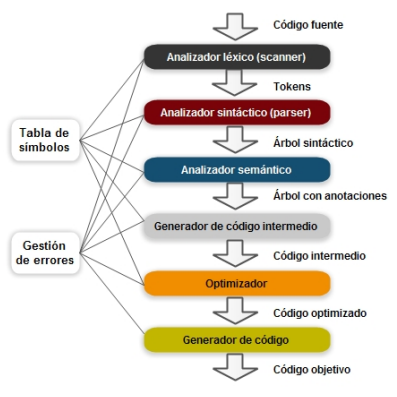
\includegraphics[width=.75\textwidth]{img/analizador_lexico.png}}
		\caption{Proceso del analizador léxico \cite{info: analizador_lexico}.}
		\label{img: analizador_lexico}
	\end{figure}
	
	Como se observa en la figura \ref{img: analizador_lexico}, el analizador tiene múltiples componentes que se encargan de:
	
	\begin{itemize}[noitemsep]
		\item Convertir el código fuente en `tokens'\footnote{Agrupación de características constituida por símbolos  que forman sentencias del lenguaje como palabras reservadas, identificadores, símbolos, etc.}.
		\item Agrupar mediante una estructura de datos tipo árbol los `tokens' para analizar la semántica.
		\item Gestiona los errores y optimiza el código generado para obtener el código objetivo.
	\end{itemize}
	
	\subsubsection{Aprendizaje automático}
	
	El aprendizaje automático (Machine Learning, ML) se centra en el desarrollo de sistemas que mejoran su rendimiento en función de los datos consumidos \cite{info: ml}. Mediante modelos de ML como clasificadores y redes neuronales, entrenados con datos etiquetados, se pueden reconocer patrones y asociarlos con fines emocionales en el contexto del PLN \cite{info: pln3}.
	
	\subsection{Salud mental}
	
	La salud mental es un estado de bienestar que permite a las personas enfrentar el estrés, desarrollar habilidades, aprender y trabajar de manera adecuada. 
	Está determinada por factores psicológicos, biológicos individuales, circunstancias sociales, económicas, políticas y ambientales. La resiliencia se ve fortalecida por interacciones sociales positivas, educación, trabajo decente, seguridad, entre otros \cite{info: salud1}.

	
	\subsubsection{Emociones}
	Las emociones son la manera natural en que los seres humanos reaccionan ante las situaciones de su entorno. Estas se presentan en diferentes intensidades a lo largo del día \cite{info: salud2}. 
	
	Las emociones pueden afectar la salud mental de formas positivas y negativas. Para tener buena salud mental es necesario equilibrar y controlar nuestras emociones. El análisis de emociones puede ser mediante las acciones o su conversación, un experto en el área puede determinar como ciertas influencias ajenas e internas alteran las emociones y por ende, la salud mental \cite{info: salud3}.
	
	\subsection{Tratamiento terapéutico psicológico}
	
	La terapia es una rama de la medicina diseñada para tratar enfermedades, mejorar la salud de los pacientes, aliviar síntomas, mejorar funciones física o psicológicas y, en caso de ser posible, erradicar la afección. La terapia puede dividirse principalmente en dos grandes grupos: farmacológico y no farmacológico. El éxito o el fracaso de cualquier terapia se ve beneficiado por un análisis preciso, seguimiento de tratamiento y participación activa del paciente \cite{info: terapia1}. 
	
	la psicología es una ciencia que estudia los procesos mentales cognitivos, afectivos y conductuales. Busca explicar el comportamiento humano para intentar predecir acciones futuras \cite{info: terapia2}.
	
	La psicoterapia es una subrama de la psicología y la terapia enfocada al tratamiento de afecciones mentales. Su objetivo es, mediante la conversación con un psicólogo o psiquiatra, aprender sobre problemas específicos, pensamientos, emociones y comportamientos que alteren el estado de animo de un individuo. Se busca que el paciente sea pueda llevar plenamente el control de su vida y que aprenda a resolver situaciones adversas.
	
	La psicoterapia puede tratar problemas mentales como:
	\begin{itemize}[noitemsep]
		\item Trastornos de ansiedad
		\item Trastornos de estados de animo
		\item Adicciones
		\item Trastornos de alimentación
		\item Trastornos de personalidad
		\item Esquizofrenia
	\end{itemize}
	
	Aunque puede ser beneficiosa con enfermedades diagnosticadas, resulta util con `conflictos' cotidianos, tales como:
	\begin{itemize}[noitemsep]
		\item Resolver conflictos
		\item Aliviar ansiedad o estrés
		\item Enfrentar cambios importantes
		\item Control de emociones
		\item Recuperación de abuso o traumas \cite{info: terapia3}
	\end{itemize}
	
	Con este proyecto se busca que, las conversaciones generadas entre el NPC y el flujo conversacional permita generar material de apoyo sobre el jugador en situaciones especificas. Este material no busca detectar enfermedades mentales ni fungir como psicólogo, busca generar un recurso que pueda ser útil para un especialista.
	
	\clearpage
	\section{Análisis}
	
	\subsection{Metodología}

	La metodología para el proyecto es el modelo de entrega por etapas. Este modelo nos permite planificar y diseñar componentes de forma individual siempre orientados a los mismos objetivos.

	El videojuego puede tener productos funcionales en las primeras etapas de desarrollo. Es por esto por lo que el modelo de entrega por etapas maximiza la productividad, permitiendo desarrollar elementos adicionales en cada una de sus etapas. 
	
	Estas implementaciones pueden ser desde niveles adicionales, mecánicas nuevas, correcciones y expansiones del mismo proyecto, permitiendo diversidad y adaptabilidad a pequeños cambios.
	
	\subsection{Tecnología}	% Herramientas, software, lenguajes de programación que seran utilizados para el desarrollo

	\subsubsection{Motor de desarrollo Unity}
	Unity es un motor y una plataforma de desarrollo de videojuegos para diseñar contenido audiovisual en 2D y 3D. Permite a programadores, artistas, arquitectos, diseñadores, cineastas, etc. diseñar, construir y desplegar sus propios proyectos en diferentes dispositivos \cite{app: unity}.

Se opta por Unity sobre otras herramientas populares en el mercado como lo son Godot, Unreal Engine y Game Maker por las siguientes razones:

\begin{itemize}
	\item Unity es el motor estandarizado para el desarrollo de proyectos nuevos, con una amplia comunidad y numerosos recursos disponibles.
	\item El juego requiere de \textit{sprites} estilo \textit{pixel art} que pueden ser segmentados y animados fácilmente mediante el IDE de Unity.
	\item El juego no requiere mucho procesamiento en los gráficos, por lo que Unity resulta una opción más cómoda y eficiente frente a Unreal Engine, que está más orientado a gráficos de alta calidad y realismo.
	\item Unity ofrece una excelente documentación y soporte técnico, lo que facilita la resolución de problemas y la implementación de características avanzadas.
	\item El editor visual de Unity es intuitivo y facilita la creación de niveles y la implementación de mecánicas de juego complejas sin requerir conocimientos avanzados en programación.
	\item Unity proporciona un excelente sistema de física y colisiones que puede ser aprovechado para crear interacciones detalladas y precisas en el juego.
\end{itemize}

	\subsubsection{Lenguaje de programación C\#}
	Lenguaje de programación utilizado comúnmente en Unity para el desarrollo de videojuegos. Es un lenguaje orientado a objetos con un sistema de gestión automática de memoria  \cite{lan: c_sharp}.
	
	\subsubsection{Lenguaje de programación Prolog}
	Lenguaje de programación basado en declaración de hechos, establecimiento de reglas e inferencias. Permite generar una base de conocimientos relacionando diferentes hechos  mediante secuencias lógicas enlazadas \cite{lan: prolog}.
	
	Su uso sera como una librería a la cual podremos acceder desde C\# para generar la base de conocimientos y la generación de inferencias. 
	
	\subsubsection{MongoDB}
	MongoDB es un sistema gestor de base de datos NoSQL orientado a documentos con estructuras BSON y esquematización dinámica.

	\begin{itemize}[noitemsep]
	\item Incluye medidas de seguridad robustas como:
		\begin{itemize}[noitemsep]
			\item \textbf{Autenticación:} Registro mediante credenciales de Atlas, GitHub o Google, lo que garantiza un acceso controlado y seguro a la base de datos.
			\item \textbf{Autorización:} Creación y asignación de roles y permisos para controlar el acceso y las operaciones que cada usuario puede realizar.
			\item \textbf{Auditoría:} Monitoreo detallado de acciones en el entorno de MongoDB, permitiendo rastrear cambios y accesos para garantizar la seguridad y el cumplimiento de normas.
			\item \textbf{Encriptación:} Protección de datos tanto en reposo como en tránsito, asegurando que la información sensible esté siempre protegida contra accesos no autorizados.
		\end{itemize}
	\item Ofrece tiempos de consulta reducidos en comparación con sistemas relacionales, lo que mejora significativamente el rendimiento en aplicaciones con grandes volúmenes de datos.
	\item Escalabilidad horizontal y vertical, permitiendo ajustar la capacidad de la base de datos según las necesidades del proyecto. Esto es especialmente útil para aplicaciones que requieren manejar grandes cantidades de datos y usuarios.
	\item Herramientas de transcripción de modelos SQL a NoSQL, facilitando la migración y la integración de bases de datos existentes.
	\item Conectividad con diferentes herramientas y sistemas de gestión, proporcionando flexibilidad y facilitando la integración con otros componentes del ecosistema tecnológico del proyecto.
	\item Integración con frameworks de desarrollo populares, lo que facilita su uso en diversas aplicaciones y entornos de desarrollo \cite{lan: mongo}.
\end{itemize}


	\subsubsection{Star UML}
	Herramienta de modelado UML desarrollado por MKLab. Es una de las herramientas UML más populares en el mundo. Se ha descargado más de 4 millones de personas y se utiliza en más de 150 países.
	
	Es compatible con los principales lenguajes de programación como Java, C\# y C ++. Puede generar códigos fuente de sus modelos o construir un modelo a partir de código fuente mediante ingeniería	inversa \cite{app: star}. 
	
	\subsubsection{Pixilart}
	Aplicación web y red social que permite diseñar, modificar, publicar y compartir imagenes estilo \textit{pixel art} de forma gratuita \cite{app: pixilart}.
	
	Esta plataforma nos permite crear grupos privados donde se puedan compartir y editar diferentes diseños. Cuenta con un amplio abanico de herramientas para colorear y dibujar en cuadricula, permitiendo formatos de alta calidad.
	
	\clearpage
	\subsection{Requerimientos}
	
	\subsubsection{Requerimientos funcionales}
	\textbf{Respecto a la jugabilidad} 
	\begin{enumerate}[label=RF\arabic*]
		\item Al iniciar, el juego muestra el menú principal con opciones para cargar partida, borrar partida, salir y acceder a la configuración.
		\item El jugador controla las acciones y las interacciones del personaje jugable.
		\item Al inicio, el juego sitúa al jugador y a un número exacto de NPCs en el \textit{respawn}.
		\item El jugador comienza un intento de progresión.
		\item Cuando el jugador inicia el intento o termina un nivel previo, el juego genera de forma procedural el siguiente nivel, compuesto por un número finito de habitaciones con obstáculos.
		\item Cuando el jugador termina el último nivel, regresa al respawn.
		\item Al finalizar cada nivel, el juego presenta una habitación con un NPC.
		\item Cuando el personaje agota sus vidas, reaparece con el último NPC con el que interactuó y entra en modo ``after'' (conservando los mismos controles), y sus estadísticas se determinan con base en el flujo de conversación.
		\item Si el personaje encuentra su lugar de muerte en modo ``after'', regresa al modo normal.
		\item Si el personaje muere en modo ``after'', vuelve al \textit{respawn} con el último NPC con el que interactuó ahí, y sus estadísticas se ajustan de acuerdo con el flujo de conversación.
	\end{enumerate}	
	
	\noindent\textbf{Respecto a la configuración}
	\begin{enumerate}[label=RF\arabic*]
		\setcounter{enumi}{10}
		\item El jugador puede configurar manualmente todos los controles o elegir la configuración predeterminada.
		\item Se permite al jugador controlar el volumen general del juego, los efectos y la música.
		\item Al terminar la interacción con un personaje, el juego guarda los datos de la partida.
		\item Al volver al menú principal, el jugador guarda los datos de la partida.
	\end{enumerate}
	
	\noindent\textbf{Respecto a los controles}
	\begin{enumerate}[label=RF\arabic*]
		\setcounter{enumi}{14}
		\item \textbf{Movimiento lateral: }El personaje puede desplazarse a lo largo del plano 2D.
		\item \textbf{Salto: }El personaje efectúa un salto vertical independiente del movimiento lateral, limitado por colisiones.
		\item \textbf{Dash: }El personaje realiza un impulso rápido en la dirección elegida por el jugador, que tiene un período de enfriamiento antes de poder reutilizarse.
	\end{enumerate}
	
	\noindent\textbf{Respecto a la interacción con el entorno}
	\begin{enumerate}[label=RF\arabic*]
		\setcounter{enumi}{17}
		\item \textbf{Conversación: }El personaje puede iniciar conversaciones con NPCs.
		\item \textbf{Finalizar conversación:} El jugador puede cerrar la ventana de diálogo con el NPC.
		\item \textbf{Cambio de escenario: }El personaje puede interactuar con puertas (o agujeros) para entrar, salir o cambiar de escenario.
		\item \textbf{Sistema de vidas: }El personaje pierde salud al colisionar con obstáculos y la recupera al completar habitaciones.
	\end{enumerate}
	
	\noindent\textbf{Respecto a la interacción con el sistema inteligente}
	\begin{enumerate}[label=RF\arabic*]
		\setcounter{enumi}{21}
		\item Cuando el jugador interactúa con un NPC, este responde según el flujo de conversación actualizado.
		\item El jugador introduce su respuesta en la conversación mediante el teclado.
		\item Con la respuesta del jugador, el juego procesa el mensaje, genera una respuesta y actualiza el flujo de conversación.
		\item El jugador tiene un número máximo de respuestas por encuentro con cada NPC.
		
	\end{enumerate}
	
	\subsubsection{Requerimientos no funcionales}
	
	\begin{enumerate}[label=RNF\arabic*]
		\item \textbf{Seguridad de Acceso: }Solo los jugadores registrados podrán acceder al juego, asegurando una experiencia segura y personalizada.
		\item \textbf{Personalización Basada en el Perfil del Jugador: }El contenido y las opciones disponibles en el juego variarán según el progreso y las acciones del jugador.
		\item \textbf{Conexión a Internet para Funcionalidades del sistema inteligente: }Se requerirá conexión a internet para acceder al servidor que contiene el sistema inteligente, permitiendo la interacción dinámica con NPC. El juego no incluirá características multiplayer online.
		\item \textbf{Mensajes de Error Claros: }Los mensajes de error serán informativos, ayudando a los desarrolladores a entender y resolver problemas rápidamente.
		\item \textbf{Diseño Adaptable a Diferentes Resoluciones y Plataformas de Escritorio:} El juego, diseñado exclusivamente para escritorio (Windows y macOS), adaptará su interfaz y gráficos a diferentes resoluciones de pantalla.
		\item \textbf{Usabilidad: }El juego será intuitivo y fácil de navegar, ofreciendo una experiencia agradable para un amplio rango de jugadores.
		\item \textbf{Terminología Amigable: }Se utilizará un lenguaje claro y accesible, evitando jerga complicada para facilitar la comprensión del juego.
		\item \textbf{Tiempo de Generación de Contenido Dinámico:} Contenidos como diálogos o eventos se generarán en menos de 10 segundos, manteniendo el flujo del juego activo.
		\item \textbf{Generación Simultánea de Contenidos: }El juego será capaz de generar múltiples elementos de juego de forma simultánea sin degradar el rendimiento.
		\item \textbf{Integridad del Contenido Generado: }Se asegurará que el contenido generado, como diálogos o eventos, sea relevante y libre de errores significativos.
		\item \textbf{Feedback Visual Durante Cargas: }Se proporcionarán indicadores de progreso durante las cargas para mantener informados a los jugadores.
		\item \textbf{Accesibilidad y Configuración de Teclado: }El juego permitirá a los usuarios configurar las teclas de acceso rápido y ajustar la sensibilidad del teclado.
		\item \textbf{Latencia Baja en la Entrada del Teclado: }Se garantizará una latencia mínima en la respuesta a las entradas del teclado.
		\item \textbf{Soporte para Atajos de Teclado: }El juego incluirá atajos de teclado intuitivos para acciones comunes.
		\item \textbf{Estilo Visual Amigable y Pixel Art: }El diseño del juego, basado en pixel art, promoverá un estilo visual amigable y atractivo, adecuado para una amplia audiencia.
		\item \textbf{Identificación Clara de Objetos y Elementos: }Tanto en el apartado visual como sonoro, los objetos y elementos importantes del juego serán fácilmente identificables, mejorando la experiencia de juego.
		\item \textbf{Juiciness en la Jugabilidad: }El juego incorpora elementos de "juiciness", ofreciendo retroalimentación inmediata y satisfactoria a las acciones del jugador a través de efectos visuales, sonoros y mecánicos que hacen que la experiencia de juego sea más dinámica y gratificante.
		
	\end{enumerate}
	
	
	\subsubsection{Requerimientos mínimos de sistema}

	\begin{table}[H]
		\centering
		\begin{tabular}{|c|l|}
			\hline
			\multicolumn{2}{|c|}{\textbf{Windows}} \\ \hline
			\textbf{Sistema operativo} & Windows  7 o mas reciente.\\ \hline
			\textbf{Procesador} &  Intel Core i3 M380. \\ \hline
			\textbf{Memoria} &  2GM de RAM. \\ \hline
			\textbf{Gráficos} &   Intel HD 4000. \\ \hline
			\textbf{DirectX} &   Versión 10. \\ \hline
			\textbf{Almacenamiento} &   1.5 GB de espacio disponible. \\ \hline
		\end{tabular}
		\caption{Requerimientos mínimos de sistema para Windows.}
		\label{table: requerimientos_windows}
	\end{table} 
	
	\begin{table}[H]
		\centering
		\begin{tabular}{|c|l|}
			\hline
			\multicolumn{2}{|c|}{\textbf{Macos}} \\ \hline
			\textbf{Sistema operativo} & Lion 10.7.5, 32/64 bits o más reciente. \\ \hline
			\textbf{Procesador} &  Intel Core i3 M380. \\ \hline
			\textbf{Memoria} &  2GM de RAM. \\ \hline
			\textbf{Gráficos} &  OpenGL 3.0 o superior. \\ \hline
			\textbf{Almacenamiento} &   1.5 GB de espacio disponible. \\ \hline
		\end{tabular}
		\caption{Requerimientos mínimos de sistema para Macos.}
		\label{table: requerimientos_mac}
	\end{table} 

	\clearpage
	\section{Diseño}
	
	\subsection{Diagrama de contexto}
	
	\begin{figure}[H]
		\centering
		\fbox{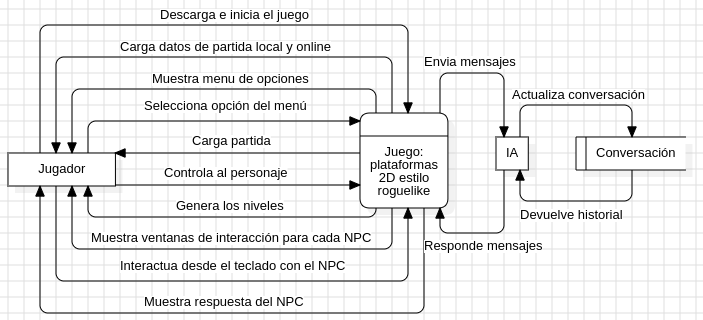
\includegraphics[width=1\textwidth]{img/contexto.png}}
		\caption{Diagrama de contexto}
		\label{diagrama: contexto}
	\end{figure}
	
	\subsection{Diagrama de flujo de datos}
	
	\begin{figure}[H]
		\centering
		\fbox{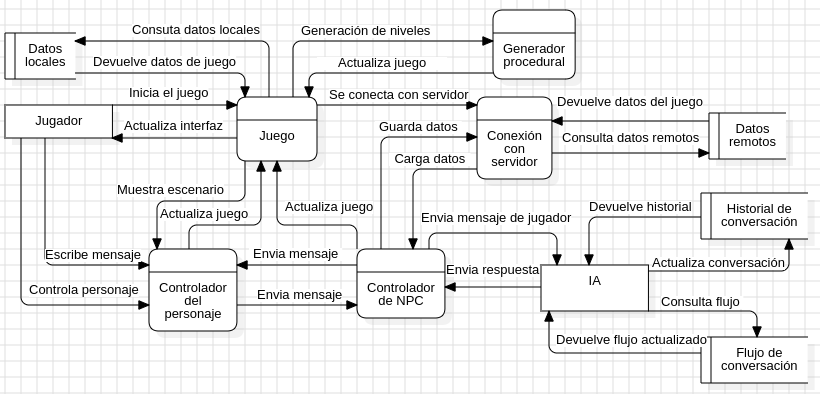
\includegraphics[width=1\textwidth]{img/flujo_datos.png}}
		\caption{Diagrama de flujo de datos}
		\label{diagrama: flujo_datos}
	\end{figure}
	
	\subsection{Diagrama de casos de uso}
	
	\begin{figure}[H]
		\centering
		\fbox{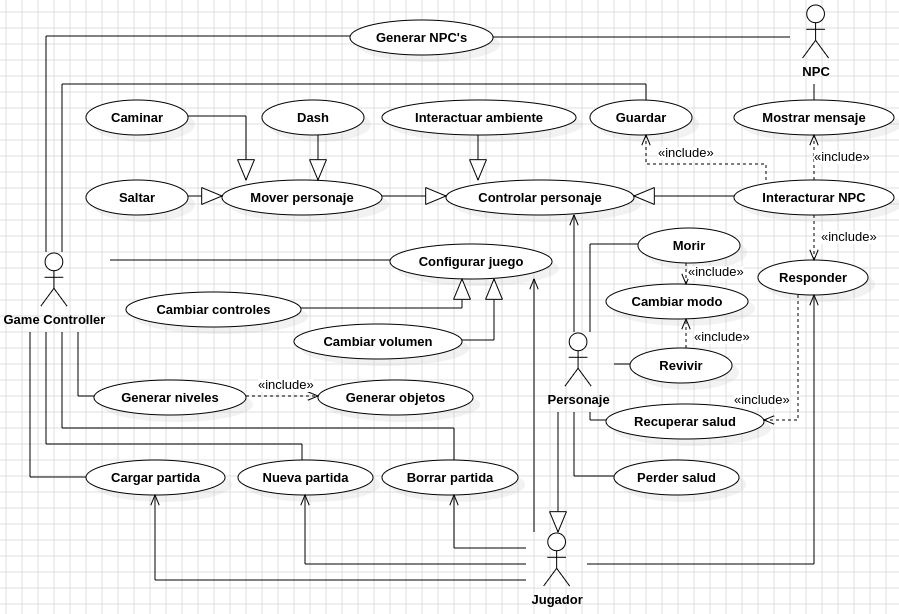
\includegraphics[width=1\textwidth]{img/casos_de_uso1.png}}
		\caption{Diagrama de casos de uso}
		\label{diagrama: casos_de_uso1}
	\end{figure}
	
	\begin{figure}[h!]
		\centering
		\fbox{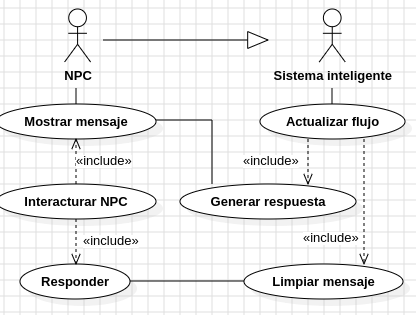
\includegraphics[width=.5\textwidth]{img/casos_de_uso2.png}}
		\caption{Diagrama de casos de uso}
		\label{diagrama: casos_de_uso2}
	\end{figure}
	
	
	
	\subsubsection{Especificaciones de casos de uso del jugador(personaje)}
	
	%Nueva partida
	\begin{figure}[H]
		\centering
		\fbox{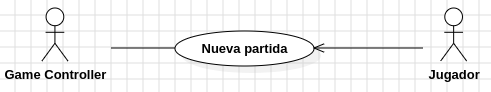
\includegraphics[width=.75\textwidth]{img/casos/nueva_partida.png}}
		\caption{Caso de uso:  Nueva partida}
		\label{diagrama: caso: nueva_partida}
	\end{figure}
	
	\begin{table}[H]
		\centering
		\begin{tabularx}{\textwidth}{|p{0.3\textwidth}|p{0.3\textwidth}|p{0.3\textwidth}|}
			\hline
			\textbf{CASO DE USO} & \multicolumn{2}{l|}{Nueva partida} \\ \hline
			
			\textbf{ACTOR} & \multicolumn{2}{l|}{Jugador} \\ \hline
			
			\textbf{DESCRIPCIÓN} & \multicolumn{2}{>{\raggedright\arraybackslash}X|}{El jugador inicia una nueva partida en un `slot' disponible.} \\ \hline
		
			\textbf{PRECONDICIÓN} & \multicolumn{2}{l|}{Ninguna} \\ \hline
			
			\textbf{FLUJO BÁSICO} & \textbf{ACTOR} & \textbf{SISTEMA} \\ \hline
			& 
			1. Presiona el botón de `Nueva partida' en el menú principal. \newline
			3. Selecciona un `slot' disponible.
			& 
			2. Muestra `slots' de almacenamiento. \newline
			4. Crea datos de partida e inicia el juego.
			\\ \hline
			
			\textbf{FLUJO ALTERNO} & \textbf{ACTOR} & \textbf{SISTEMA} \\ \hline
			
			1. Sin `slots' de almacenamiento: Cancelar.
			& 
			1. Presiona el botón de `Nueva partida' en el menú principal. \newline
			3. Selecciona un `slot' no disponible. \newline
			5. Selecciona la opción de cancelar.
			&
			2. Muestra `slots' de almacenamiento. \newline
			4. Mensaje de advertencia para sobrescribir datos o cancelar. \newline
			6. Regresa al menú principal.
			\\ \hline
			
			\textbf{FLUJO ALTERNO} & \textbf{ACTOR} & \textbf{SISTEMA} \\ \hline
			
			2. Sin `slots' de almacenamiento: Cancelar.
			& 
			1. Presiona el botón de `Nueva partida' en el menú principal. \newline
			3. Selecciona un `slot' no disponible. \newline
			5. Selecciona la opción de sobrescribir.
			&
			2. Muestra `slots' de almacenamiento. \newline
			4. Mensaje de advertencia para sobrescribir datos o cancelar. \newline
			6. Borra datos de partida pasada, crea datos de partida e inicia el juego.
			\\ \hline
			
			\textbf{POSTCONDICIÓN} & \multicolumn{2}{l|}{Ninguna} \\ \hline
		\end{tabularx}
		\caption{Descripción del caso de uso: Nueva partida.}
		\label{table:caso_nueva_partida}
	\end{table}
	
	%Cargar partida
	\begin{figure}[H]
		\centering
		\fbox{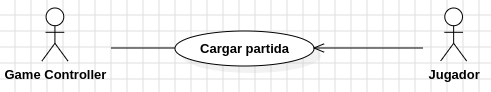
\includegraphics[width=.75\textwidth]{img/casos/cargar_partida.png}}
		\caption{Caso de uso: Cargar partida}
		\label{diagrama: caso: cargar_partida}
	\end{figure}
	
	\begin{table}[H]
		\centering
		\begin{tabularx}{\textwidth}{|p{0.3\textwidth}|p{0.3\textwidth}|p{0.3\textwidth}|}
			\hline
			\textbf{CASO DE USO} & \multicolumn{2}{l|}{Cargar partida} \\ \hline
			
			\textbf{ACTOR} & \multicolumn{2}{l|}{Jugador} \\ \hline
			
			\textbf{DESCRIPCIÓN} & \multicolumn{2}{>{\raggedright\arraybackslash}X|}{El jugador carga los datos de la partida guardada e inicia el juego.} \\ \hline
			
			\textbf{PRECONDICIÓN} & \multicolumn{2}{l|}{Nueva partida} \\ \hline
			
			\textbf{FLUJO BÁSICO} & \multicolumn{1}{c|}{\textbf{ACTOR}} & \multicolumn{1}{c|}{\textbf{SISTEMA} } \\ \hline
			& 
			1. Selecciona el `slot' de partida.
			&
			2. Carga datos de partida, e inicia el juego.
			 \\ \hline
			
			\textbf{POSTCONDICIÓN} & \multicolumn{2}{l|}{Ninguna} \\ \hline
		\end{tabularx}
		\caption{Descripción del caso de uso: Cargar partida }
		\label{table: caso: cargar_partida}
	\end{table}
	
	%Borrar partida
	\begin{figure}[H]
		\centering
		\fbox{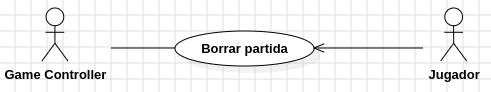
\includegraphics[width=.75\textwidth]{img/casos/borrar_partida.png}}
		\caption{Caso de uso: Borrar partida.}
		\label{diagrama: caso: borrar_partida}
	\end{figure}
	
	\begin{table}[H]
		\centering
		\begin{tabularx}{\textwidth}{|p{0.3\textwidth}|p{0.3\textwidth}|p{0.3\textwidth}|}
			\hline
			\textbf{CASO DE USO} & \multicolumn{2}{l|}{Borrar partida} \\ \hline
			
			\textbf{ACTOR} & \multicolumn{2}{l|}{Jugador} \\ \hline
			
			\textbf{DESCRIPCIÓN} & \multicolumn{2}{>{\raggedright\arraybackslash}X|}{El jugador elimina los datos guardados de una partida.} \\ \hline
			
			\textbf{PRECONDICIÓN} & \multicolumn{2}{l|}{Nueva partida} \\ \hline
			
			\textbf{FLUJO BÁSICO} & \multicolumn{1}{c|}{\textbf{ACTOR}} & \multicolumn{1}{c|}{\textbf{SISTEMA} } \\ \hline
			& 
			1. Selecciona el botón de eliminar `slot' de partida. \newline
			3. Selecciona eliminar los datos.
			&
			2. Mensaje de advertencia para eliminar o cancelar. \newline
			4. Elimina permanente los datos de partida del `slot'.
			 \\ \hline
			
			\textbf{FLUJO ALTERNO} & \multicolumn{1}{c|}{\textbf{ACTOR}} & \multicolumn{1}{c|}{\textbf{SISTEMA} } \\ \hline
			
			1. Cancelar.
			& 
			1. Selecciona el botón de eliminar `slot' de partida. \newline
			3. Selecciona cancelar.
			&
			2. Mensaje de advertencia para eliminar o cancelar. \newline
			4. Regresa al menú principal.
			\\ \hline
			
			
			\textbf{POSTCONDICIÓN} & \multicolumn{2}{l|}{Ninguna} \\ \hline
		\end{tabularx}
		\caption{Descripción del caso de uso: Eliminar partida}
		\label{table: caso: eliminar_partida}
	\end{table}
	
	%Cambiar controles
	\begin{figure}[H]
		\centering
		\fbox{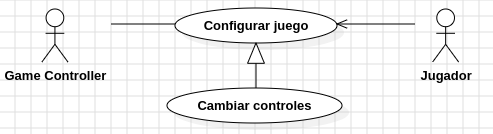
\includegraphics[width=.75\textwidth]{img/casos/cambiar_controles.png}}
		\caption{Caso de uso: Cambiar controles}
		\label{diagrama: caso: cambiar_controles}
	\end{figure}
	
	\begin{table}[H]
		\centering
		\begin{tabularx}{\textwidth}{|p{0.3\textwidth}|p{0.3\textwidth}|p{0.3\textwidth}|}
			\hline
			\textbf{CASO DE USO} & \multicolumn{2}{l|}{Cambiar controles} \\ \hline
			
			\textbf{ACTOR} & \multicolumn{2}{l|}{Jugador} \\ \hline
			
			\textbf{DESCRIPCIÓN} & \multicolumn{2}{>{\raggedright\arraybackslash}X|}{El jugador configura los controles para las acciones del personaje.} \\ \hline
			
			\textbf{PRECONDICIÓN} & \multicolumn{2}{l|}{Ninguna} \\ \hline
			
			\textbf{FLUJO BÁSICO} & \multicolumn{1}{c|}{\textbf{ACTOR}} & \multicolumn{1}{c|}{\textbf{SISTEMA} } \\ \hline
			& 
			1. Selecciona el menú de configuración. \newline
			3. Selecciona el sub menú de controles. \newline
			5. Selecciona una acción. \newline
			7. Presiona un botón en el tiempo dado. \
			&
			2. Muestra configuración de audio y de controles. \newline
			4. Muestra un listado de acciones y su botón/tecla asignada. \newline
			6. Inicia un contador esperando respuesta del jugador. \newline 
			8. Configura la acción al botón seleccionado. 
			 \\ \hline
			 
			 \textbf{FLUJO ALTERNO} & \multicolumn{1}{c|}{\textbf{ACTOR}} & \multicolumn{1}{c|}{\textbf{SISTEMA} } \\ \hline
			 1. Omisión.
			 & 
			 1. Selecciona el menú de configuración. \newline
			 3. Selecciona el sub menú de controles. \newline
			 5. Selecciona una acción. \newline
			 7. No presiona un botón en el tiempo dado. 
			 &
			 2. Muestra configuración de audio y de controles. \newline
			 4. Muestra un listado de acciones y su botón/tecla asignada. \newline
			 6. Inicia un contador esperando respuesta del jugador. \newline 
			 8. Mantiene la configuración actual de la acción. 
			 \\ \hline
			
			\textbf{POSTCONDICIÓN} & \multicolumn{2}{l|}{Ninguna} \\ \hline
		\end{tabularx}
		\caption{Descripción del caso de uso: Cambiar controles}
		\label{table: caso: cambiar_controles}
	\end{table}
	
	%cambiar volumen
	\begin{figure}[H]
		\centering
		\fbox{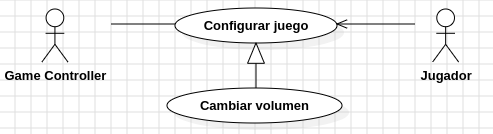
\includegraphics[width=.75\textwidth]{img/casos/cambiar_volumen.png}}
		\caption{Caso de uso: Cambiar volumen}
		\label{diagrama: caso: cambiar_volumen}
	\end{figure}
	
	\begin{table}[H]
		\centering
		\begin{tabularx}{\textwidth}{|p{0.3\textwidth}|p{0.3\textwidth}|p{0.3\textwidth}|}
			\hline
			\textbf{CASO DE USO} & \multicolumn{2}{l|}{Cambiar volumen} \\ \hline
			
			\textbf{ACTOR} & \multicolumn{2}{l|}{Jugador} \\ \hline
			
			\textbf{DESCRIPCIÓN} & \multicolumn{2}{>{\raggedright\arraybackslash}X|}{Se configuran los volúmenes del juego} \\ \hline
			
			\textbf{PRECONDICIÓN} & \multicolumn{2}{l|}{Ninguna} \\ \hline
			
			\textbf{FLUJO BÁSICO} & \multicolumn{1}{c|}{\textbf{ACTOR}} & \multicolumn{1}{c|}{\textbf{SISTEMA} } \\ \hline
			&
			1. Selecciona el menú de configuración. \newline
			3. Selecciona el sub menú de volumen. \newline
			5. Selecciona y desplaza la barra de volumen especifica. 
			& 
			2. Muestra configuración de audio y de controles. \newline
			4. Muestra barras deslizables de volumen. \newline
			6. Actualiza el volumen seleccionado. 
			\\ \hline
			
			\textbf{POSTCONDICIÓN} & \multicolumn{2}{l|}{Ninguna} \\ \hline
		\end{tabularx}
		\caption{Descripción del caso de uso: Cambiar volumen}
		\label{table: caso: cambiar_volumen}
	\end{table}
	
	% Cambiar modo
	\begin{figure}[H]
		\centering
		\fbox{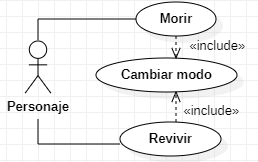
\includegraphics[width=.5\textwidth]{img/casos/cambiar_modo.png}}
		\caption{Caso de uso: Cambiar modo}
		\label{diagrama: caso: cambiar_modo}
	\end{figure}
	
	\begin{table}[H]
		\centering
		\begin{tabularx}{\textwidth}{|p{0.3\textwidth}|p{0.3\textwidth}|p{0.3\textwidth}|}
			\hline
			\textbf{CASO DE USO} & \multicolumn{2}{l|}{Cambiar modo} \\ \hline
			
			\textbf{ACTOR} & \multicolumn{2}{l|}{Personaje (Jugador)} \\ \hline
			
			\textbf{DESCRIPCIÓN} & \multicolumn{2}{>{\raggedright\arraybackslash}X|}{El personaje tiene un segundo intento después de morir y lo recupera cuando revive} \\ \hline
			
			\textbf{PRECONDICIÓN} & \multicolumn{2}{l|}{Morir o Revivir} \\ \hline
			
			\textbf{FLUJO BÁSICO} & \multicolumn{1}{c|}{\textbf{ACTOR}} & \multicolumn{1}{c|}{\textbf{SISTEMA} } \\ \hline
			&
			1. El personaje muere. \newline 
			2. El personaje encuentra el lugar donde falleció. 
			& 
			2. El personaje reaparece con el ultimo NPC con el que interactuó (Sus estadísticas están determinadas por el flujo conversacional del NPC) en modo `after'. \newline
			3. El personaje recupera sus estadísticas iniciales y continua el juego. 
			\\ \hline
			
			\textbf{FLUJO ALTERNO} & \multicolumn{1}{c|}{\textbf{ACTOR}} & \multicolumn{1}{c|}{\textbf{SISTEMA} } \\ \hline
			1. El jugador fallece en modo `after'.
			&
			1. El personaje muere. \newline 
			2. El personaje muere nuevamente. 
			& 
			2. El personaje reaparece con el ultimo NPC con el que interactuó en modo `after'. \newline
			3. El personaje reaparece en el `respawn'.
			\\ \hline
			
			\textbf{FLUJO ALTERNO} & \multicolumn{1}{c|}{\textbf{ACTOR}} & \multicolumn{1}{c|}{\textbf{SISTEMA} } \\ \hline
			1. El jugador no fallece en modo `after' y no encuentra donde falleció.
			&
			1. El personaje muere. \newline 
			2. El personaje sigue jugando en modo `after'.
			& 
			2. El personaje reaparece con el ultimo NPC con el que interactuó en modo `after'. \newline
			3. El personaje se mantiene en modo `after'.
			\\ \hline
			
			
			\textbf{POSTCONDICIÓN} & \multicolumn{2}{l|}{Revivir o Morir} \\ \hline
		\end{tabularx}
		\caption{Descripción del caso de uso: Cambiar modo}
		\label{table: caso: cambiar_modo}
	\end{table}
	
	%Perder salud
	\begin{figure}[H]
		\centering
		\fbox{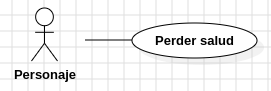
\includegraphics[width=.5\textwidth]{img/casos/perder_salud.png}}
		\caption{Caso de uso: Perder salud}
		\label{diagrama: caso: perder_salud}
	\end{figure}
	
	\begin{table}[H]
		\centering
		\begin{tabularx}{\textwidth}{|p{0.3\textwidth}|p{0.3\textwidth}|p{0.3\textwidth}|}
			\hline
			\textbf{CASO DE USO} & \multicolumn{2}{l|}{Perder salud} \\ \hline
			
			\textbf{ACTOR} & \multicolumn{2}{l|}{Personaje (Jugador)} \\ \hline
			
			\textbf{DESCRIPCIÓN} & \multicolumn{2}{>{\raggedright\arraybackslash}X|}{El jugador pierde puntos de vida al sufrir daño.} \\ \hline
			
			\textbf{PRECONDICIÓN} & \multicolumn{2}{l|}{Ninguna.} \\ \hline
			
			\textbf{FLUJO BÁSICO} & \multicolumn{1}{c|}{\textbf{ACTOR}} & \multicolumn{1}{c|}{\textbf{SISTEMA} } \\ \hline
			&
			1. Choca con un obstáculo.
			& 
			2. Se disminuye un punto de vida y el personaje regresa al inicio de la habitación. 
			\\ \hline
			
			\textbf{FLUJO ALTERNO} & \multicolumn{1}{c|}{\textbf{ACTOR}} & \multicolumn{1}{c|}{\textbf{SISTEMA} } \\ \hline
			1. Vida mínima.
			&
			1. Choca con un obstáculo.
			& 
			2. Fallece y cambia a modo `after'. 
			\\ \hline
			
			
			\textbf{POSTCONDICIÓN} & \multicolumn{2}{l|}{Morir} \\ \hline
		\end{tabularx}
		\caption{Descripción del caso de uso: }
		\label{table: caso: }
	\end{table}

	%Recuperar salud
	\begin{figure}[H]
		\centering
		\fbox{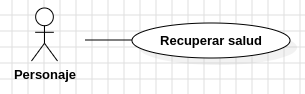
\includegraphics[width=.5\textwidth]{img/casos/recuperar_salud.png}}
		\caption{Caso de uso: Recuperar salud}
		\label{diagrama: caso: recuperar_salud}
	\end{figure}
	
	\begin{table}[H]
		\centering
		\begin{tabularx}{\textwidth}{|p{0.3\textwidth}|p{0.3\textwidth}|p{0.3\textwidth}|}
			\hline
			\textbf{CASO DE USO} & \multicolumn{2}{l|}{Recuperar salud} \\ \hline
			
			\textbf{ACTOR} & \multicolumn{2}{l|}{Personaje (Jugador)} \\ \hline
			
			\textbf{DESCRIPCIÓN} & \multicolumn{2}{>{\raggedright\arraybackslash}X|}{Aumenta los puntos de vida de personaje cada que termina una habitación.} \\ \hline
			
			\textbf{PRECONDICIÓN} & \multicolumn{2}{l|}{Ninguna} \\ \hline
			
			\textbf{FLUJO BÁSICO} & \multicolumn{1}{c|}{\textbf{ACTOR}} & \multicolumn{1}{c|}{\textbf{SISTEMA} } \\ \hline
			& 
			1. El jugador termina una habitación.
			&
			2. Adquiere un punto de vida. 
			\\ \hline
			
			\textbf{FLUJO ALTERNO} & \multicolumn{1}{c|}{\textbf{ACTOR}} & \multicolumn{1}{c|}{\textbf{SISTEMA} } \\ \hline
			1. Vida máxima.
			& 
			1. El jugador termina una habitación.
			&
			2. No recibe puntos adicionales de vida.
			\\ \hline
			
			\textbf{POSTCONDICIÓN} & \multicolumn{2}{l|}{Ninguna.} \\ \hline
		\end{tabularx}
		\caption{Descripción del caso de uso: Recuperar salud}
		\label{table: caso: recuperar_salud}
	\end{table}
		
	%Caminar
	\begin{figure}[H]
		\centering
		\fbox{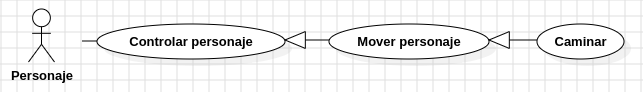
\includegraphics[width=\textwidth]{img/casos/caminar.png}}
		\caption{Caso de uso: Caminar}
		\label{diagrama: caso: caminar}
	\end{figure}
	
	\begin{table}[H]
		\centering
		\begin{tabularx}{\textwidth}{|p{0.3\textwidth}|p{0.3\textwidth}|p{0.3\textwidth}|}
			\hline
			\textbf{CASO DE USO} & \multicolumn{2}{l|}{Caminar} \\ \hline
			
			\textbf{ACTOR} & \multicolumn{2}{l|}{Personaje (Jugador)} \\ \hline
			
			\textbf{DESCRIPCIÓN} & \multicolumn{2}{>{\raggedright\arraybackslash}X|}{El jugador se mueve en el eje horizontal.} \\ \hline
			
			\textbf{PRECONDICIÓN} & \multicolumn{2}{l|}{Ninguna.} \\ \hline
			
			\textbf{FLUJO BÁSICO} & \multicolumn{1}{c|}{\textbf{ACTOR}} & \multicolumn{1}{c|}{\textbf{SISTEMA} } \\ \hline
			& 
			1. El jugador presiona las teclas de movimiento horizontal.
			& 
			2. El personaje se mueve en la dirección seleccionada.
			\\ \hline
			
			\textbf{FLUJO ALTERNO} & \multicolumn{1}{c|}{\textbf{ACTOR}} & \multicolumn{1}{c|}{\textbf{SISTEMA} } \\ \hline
			1. Colisión.
			& 
			1. El jugador presiona las teclas de movimiento horizontal. \newline
			3. El personaje alcanza un muro. 
			& 
			2. El personaje se mueve en la dirección seleccionada.\newline
			4. El personaje colisiona y detiene el movimiento. 
			\\ \hline
			
			\textbf{POSTCONDICIÓN} & \multicolumn{2}{l|}{Ninguna} \\ \hline
		\end{tabularx}
		\caption{Descripción del caso de uso: Caminar}
		\label{table: caso: caminar}
	\end{table}
	
	%Saltar
	\begin{figure}[H]
		\centering
		\fbox{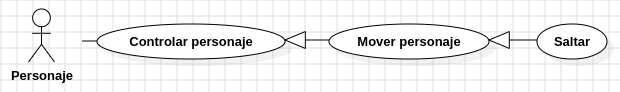
\includegraphics[width=.75\textwidth]{img/casos/saltar.png}}
		\caption{Caso de uso: Saltar}
		\label{diagrama: caso: saltar}
	\end{figure}
	
	\begin{table}[H]
		\centering
		\begin{tabularx}{\textwidth}{|p{0.3\textwidth}|p{0.3\textwidth}|p{0.3\textwidth}|}
			\hline
			\textbf{CASO DE USO} & \multicolumn{2}{l|}{Saltar} \\ \hline
			
			\textbf{ACTOR} & \multicolumn{2}{l|}{Personaje (Jugador)} \\ \hline
			
			\textbf{DESCRIPCIÓN} & \multicolumn{2}{>{\raggedright\arraybackslash}X|}{El personaje realiza un salto vertical mediante un impulso. } \\ \hline
			
			\textbf{PRECONDICIÓN} & \multicolumn{2}{l|}{Ninguna.} \\ \hline
			
			\textbf{FLUJO BÁSICO} & \multicolumn{1}{c|}{\textbf{ACTOR}} & \multicolumn{1}{c|}{\textbf{SISTEMA} } \\ \hline
			&
			1. El personaje esta tocando el suelo y presiona la tecla para saltar.  
			& 
			2. Cambio de posición vertical mediante un impulso (curva parabólica). 
			\\ \hline
			
			\textbf{FLUJO ALTERNO} & \multicolumn{1}{c|}{\textbf{ACTOR}} & \multicolumn{1}{c|}{\textbf{SISTEMA} } \\ \hline
			1. Colisión.
			&
			1. El personaje esta tocando el suelo y presiona la tecla para saltar.  \newline
			3. El personaje alcanza un muro(techo).
			& 
			2. Cambio de posición vertical mediante un impulso (curva parabólica). \newline
			4. Se cancela la velocidad vertical del personaje para empezar su descenso. 		
			\\ \hline
			
			\textbf{FLUJO ALTERNO} & \multicolumn{1}{c|}{\textbf{ACTOR}} & \multicolumn{1}{c|}{\textbf{SISTEMA} } \\ \hline
			2. Permisión de salto.
			& 
			1. El personaje se encuentra en el aire. \newline
			3. Toca una superficie de piso. 
			& 
			2. Se inhabilita el salto. \newline
			4. Se habilita el salto.
			\\ \hline
			
			\textbf{POSTCONDICIÓN} & \multicolumn{2}{|l|}{Ninguna} \\ \hline
		\end{tabularx}
		\caption{Descripción del caso de uso: Saltar}
		\label{table: caso: saltar}
	\end{table}
	
	%Responder
	\begin{figure}[H]
		\centering
		\fbox{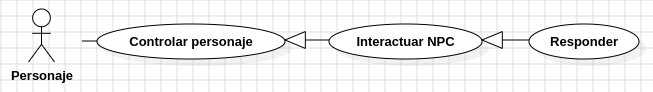
\includegraphics[width=.75\textwidth]{img/casos/responder.png}}
		\caption{Caso de uso: Responder}
		\label{diagrama: caso: responder}
	\end{figure}
	
	\begin{table}[H]
		\centering
		\begin{tabularx}{\textwidth}{|p{0.3\textwidth}|p{0.3\textwidth}|p{0.3\textwidth}|}
			\hline
			\textbf{CASO DE USO} & \multicolumn{2}{l|}{Responder} \\ \hline
			
			\textbf{ACTOR} & \multicolumn{2}{l|}{personaje (Jugador)} \\ \hline
			
			\textbf{DESCRIPCIÓN} & \multicolumn{2}{>{\raggedright\arraybackslash}X|}{El jugador responde el mensaje del NPC desde el teclado. } \\ \hline
			
			\textbf{PRECONDICIÓN} & \multicolumn{2}{l|}{NPC: mostrar mensaje} \\ \hline
			
			\textbf{FLUJO BÁSICO} & \multicolumn{1}{c|}{\textbf{ACTOR}} & \multicolumn{1}{c|}{\textbf{SISTEMA} } \\ \hline
			& 
			1. El jugador escribe el mensaje y lo envía.
			& 
			2. Se envía el mensaje al sistema inteligente e imprime una respuesta. 
			\\ \hline
			
			\textbf{FLUJO ALTERNO} & \multicolumn{1}{c|}{\textbf{ACTOR}} & \multicolumn{1}{c|}{\textbf{SISTEMA} } \\ \hline
			1. Cancelación.
			& 
			1. El jugador escribe el mensaje y cierra la ventana de dialogo.
			& 
			2. Cierra la ventana de dialogo y regresa al juego.
			\\ \hline
			
			\textbf{POSTCONDICIÓN} & \multicolumn{2}{l|}{Ninguna.} \\ \hline
		\end{tabularx}
		\caption{Descripción del caso de uso: Responder}
		\label{table: caso: responder}
	\end{table}
	
	
	\clearpage
	\subsection{Diagrama de clases}

	Con base en el genero del videojuego, se requiere de diferentes clases que complementen la funcionalidad lógica. Elementos como la cámara, `sprites', colisiones, sonidos, partículas, animaciones, cinemáticas, etc. pueden ser añadidas directo desde el IDE de Unity. Por esta razón, el diagrama de clases de la figura \ref{diagrama: clases} omite esos aspectos de construcción (constructores, `getters' y `setters' incluidos) y busca representar la estructura y relación entre clases.

	\begin{figure}[H]
		\centering
		\fbox{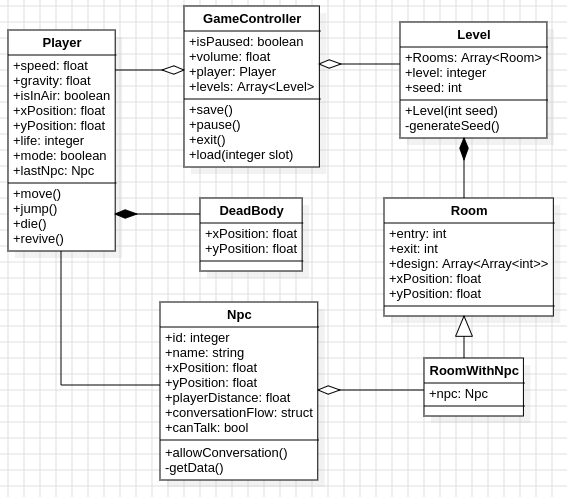
\includegraphics[width=\textwidth]{img/clases.png}}
		\caption{Diagrama de clases}
		\label{diagrama: clases}
	\end{figure}
	
	\clearpage
	
	\section{Conclusiones}
	
	En esta primera etapa del proyecto, se logró establecer la estructura básica fundamental para el desarrollo del videojuego. Se alcanzaron varios hitos importantes que sientan las bases para las etapas subsiguientes:
	
	\begin{itemize}
		\item Se implementó con éxito el controlador del personaje, que incluye animaciones fluidas, efectos visuales y un sistema de movimiento que responde de manera intuitiva a las acciones del jugador.
		\item Se desarrolló un controlador funcional para los NPCs, permitiendo su generación dentro de los niveles y la interacción no procedural con el jugador. Esto establece las primeras interacciones y dinámicas básicas entre el personaje principal y los personajes no jugables.
		\item Se diseñó y probó un modelo inicial para la construcción de habitaciones, lo que facilita la creación y la implementación de diversos diseños de habitaciones que enriquecerán la experiencia del juego.
		\item Se implementó un generador de niveles que utiliza semillas o claves únicas para generar entornos y paisajes de manera procedural, asegurando así experiencias de juego únicas y variadas en cada partida.
		\item Se avanzó significativamente en la creación del entorno visual y artístico del juego, sentando las bases estéticas y de diseño que capturan la esencia y la atmósfera deseada para el juego final.
	\end{itemize}
	
	Para las próximas etapas del desarrollo, se planea enfocarse en la implementación de controladores adicionales para la configuración del juego, permitiendo ajustes dinámicos y mejoras en la jugabilidad. Además, se buscará expandir la variedad de habitaciones disponibles, diseñar nuevos niveles desafiantes, introducir personajes adicionales con comportamientos distintivos y mejorar continuamente los diseños gráficos para ofrecer una experiencia visualmente cautivadora y cohesiva.
	
	Estas metas futuras no solo enriquecerán el contenido y la complejidad del juego, sino que también asegurarán que el proyecto avance hacia su objetivo final de crear un videojuego \textit{rogue lite} innovador y atractivo para los jugadores.

	
	\clearpage
	
	\section{Referencias Bibliográficas}
	
	\begin{thebibliography}{10}
	
	%Estado del arte
	\bibitem{game: hades}
	Supergiant Games, \textit{Hades}. Supergiant Games, 2019.
	
	\bibitem{game: celeste}
	Maddy Makes Games, \textit{Celeste}. Maddy Makes Games, 2018.
	
	\bibitem{game: hollow}
	Team Cherry, \textit{Hollow Knight}. Team Cherry, 2017.
	
	\bibitem{game: coffee}
	Toge Productions, \textit{Coffee Talk}. Toge Productions, 2020.
	
	\bibitem{app: character}
	Character Technologies, Inc. ``character.ai'', 2022. [En línea]. Disponible: \url{https://character.ai}. [Accedido: 11-Junio-2024].
	
	\bibitem{info: justificacion1}
	Secretaria de salud, ``Depresión y ansiedad, principales problemas de salud mental en estos segmentos poblacionales'', Gobierno de México. [En línea]. Disponible: \url{https://www.gob.mx/salud/prensas}. [Accedido: 23-Junio-2024].
	
	\bibitem{info: justificacion2}
	Gonzáles Mario, ``Cómo se aplica la Inteligencia Artificial en los videojuegos'', Instituto de ingeniería del conocimiento. [En línea]. Disponible: \url{https://www.iic.uam.es/noticias/como-aplica-inteligencia-artificial-en-videojuegos/}. [Accedido: 23-junio-2024].
	
	\bibitem{info: justificacion3}
	Hernández Cabezas Ariadna, ``Videojuegos como tratamiento terapéutico'', [En línea]. Disponible: \url{https://repositori.uji.es/xmlui/bitstream/handle/10234/191101/TFM_2020_HernandezCabezas_Ariadna.pdf?sequence=1&isAllowed=y} [Accedido: 23-junio-2024].
	
	\bibitem{info: videojuego1}
	Salinaz Benito, ``UDLAP'', catarina. [En línea]. Disponible: \url{http://catarina.udlap.mx/u_dl_a/tales/documentos/lnd/benitez_salinas_ve/capitulo1.pdf}. [Accedido: 20-Junio-2024].
	
	\bibitem{info: videojuego2}
	Plarium, ``Roguelike''. [En línea]. Disponible: \url{https://plarium.com/es/glossary/roguelike-games/}. [Accedido: 20-Junio-2024].
	
	\bibitem{info: pln1}
	Google Cloud, ``¿Qué es el procesamiento del lenguaje natural?''. [En línea]. Disponible: \url{https://cloud.google.com/learn/what-is-natural-language-processing}. [Accedido: 20-Junio-2024].
	
	\bibitem{info: def: polisemica}
	Real Academia Española, ``polisémico, ca''. [En línea]. Disponible: \url{https://www.rae.es/diccionario-estudiante/polisémico}. [Accedido: 20-Junio-2024].
	
	\bibitem{info: def: homonimo}
	Real Academia Española, ``homónimo, ma''. [En línea]. Disponible: \url{https://dle.rae.es/homónimo}. [Accedido: 20-Junio-2024].
	
	\bibitem{info: pln2}
	IMB, ``¿Qué es el procesamiento del lenguaje natural (NLP)?''. [En línea]. Disponible: \url{https://www.ibm.com/mx-es/topics/natural-language-processing}. [Accedido: 20-Junio-2024].
	
	\bibitem{info: pln3}
	Prompts para IA, ``Procesamiento del lenguaje natural y detección de emociones'', 2024. [En línea]. Disponible: \url{https://prompt.uno/vision-por-computadora/procesamiento-del-lenguaje-natural-y-deteccion-de-emociones/}. [Accedido: 20-Junio-2024].
	
	\bibitem{info: analizador_lexico}
	Universidad Europea de Madrid, S.L.U, ``'Análisis léxico''', Cartagena99. [En línea]. Disponible: \url{https://www.cartagena99.com/recursos/alumnos/apuntes/ININF2_M4_U2_T1.pdf}. [Accedido: 20-Junio-2024].
	
	\bibitem{info: ml}
	Oracle, ``¿Qué es el machine learning?''. [En línea]. Disponible: \url{https://www.oracle.com/mx/artificial-intelligence/machine-learning/what-is-machine-learning/}. [Accedido: 20-Junio-2024].
	
	\bibitem{info: salud1}
	Organización Mundial de la Salud, ``Salud mental: fortalecer neustra respuesta'', 17-Junio-2022. [En línea]. Disponible: \url{https://www.who.int/es/news-room/fact-sheets/detail/mental-health-strengthening-our-response}. [Accedido: 20-Junio-2024].
	
	\bibitem{info: salud2}
	Unicef, ``Cómo reconocer nuestras emociones''. [En línea]. Disponible: \url{https://www.unicef.org/lac/crianza/seguridad-proteccion/como-reconocer-nuestras-emociones}. [Accedido: 20-Junio-2024].
	
	\bibitem{info: salud3}
	Arancibia Psicología, ``La relación entre las emociones y la salud mental''. [En línea]. Disponible: \url{https://www.arancibia-psicologia.com}. [Accedido: 20-Junio-2024].
	
	\bibitem{info: terapia1}
	Clinica Universidad de Navarra, ``Terapia''. [En línea]. Disponible: \url{https://www.cun.es/diccionario-medico/terminos/terapia}. [Accedido: 22-Junio-2024].
	
	\bibitem{info: terapia2}
	Definición, ``Psicología''. [En línea]. Disponible: \url{https://definicion.de/psicologia/}. [Accedido: 22-Junio-2024].
	
	\bibitem{info: terapia3}
	Mayo Clinic, ``Psicoterapia''. [En línea]. Disponible: \url{https://www.mayoclinic.org/es/tests-procedures/psychotherapy/about/pac-20384616}. [Accedido: 22-Junio-2024].
	
	\bibitem{app: unity}
	Unity Technologies. ``Unity para principiantes | Unity''. Unity. [En línea]. Disponible: \url{https://unity.com/es/learn/get-started}. [Accedido: 13-Junio-2024].
	
	\bibitem{lan: c_sharp}
	E. Canle Fernández, ``¿Qué lenguaje de programación usa Unity? – Tokio School''. Tokio School. [En línea]. Disponible: \url{https://www.tokioschool.com/noticias/lenguaje-unity}. [Accedido: 13-Junio-2024].
	
	\bibitem{lan: prolog}
	UNAM, ``PROLOG''. [En línea]. Disponible: \url{https://virtual.cuautitlan.unam.mx/intar}. [Accedido: 13-Junio-2024].
	
	\bibitem{lan: mongo}
	MongoDB, ``MongoDB: The Developer Data Platform''. MongoDB. [En línea]. Disponible: \url{https://www.mongodb.com}. [Accedido: 13-Junio-2024].
	
	\bibitem{app: star}
	MKLab, ``StarUML''. StarUML. [En línea]. Disponible: \url{https://www.pixilart.com}. [Accedido: 13-Junio-2024].
	
	\bibitem{app: pixilart}
	Pixilart, ``Pixilart''. Pixilart LLC. [En línea]. Disponible: \url{https://staruml.io}. [Accedido: 13-Junio-2024].
	

	\end{thebibliography}
	
\end{document}

